\chapter{Simulations}
\section{Introduction}
\label{sec:Simulations:Intro}

The purpose of performing simulations and analysing their results is to explore the efficacy of each agent's strategy under different conditions. We would like to answer questions such as: 

\begin{itemize}
    \item Does the benefit of running the IIGO outweigh its cost? 
    \item Can the agent strategies overcome the foraging dilemma outlined in Section INSERT REF LATER? 
    \item Do the agents act selflessly or selfishly?
    \item How important is collaboration to an island's survival?
    \item How do the island's organise themselves under different conditions? %maybe change
\end{itemize}

The analysis encapsulates the purpose of the entire coursework and therefore, is the final result of all the work done. In this chapter, we aim to prove that our platform and the agents are capable of displaying interesting behaviour and hence, we can draw conclusions about how certain behaviours and environmental factors affect a multi-agent system.

\section{Metrics}
\label{sec:Simulations:Metric}

To assist in this analysis, we need to draw quantifiable results from the simulations. Thus enters the metrics: These numerical values give us information on the events of the game that we can then use to compare numerous simulations and draw insights into what influences the changing of certain parameters has on the game. Some metrics are also worth knowing on a turn by turn basis and as such have been represented as graphs. 


\begin{itemize}
    \item \textbf{Archipelago Survivability}: Number of turns until all the islands in the archipelago die.
    \item \textbf{First Island Death}: Number of turns until any island dies.
    \item \textbf{Island Resources\footnote{\label{foot:Simulations:per_island}Presented on a per-island basis.}\footnote{\label{foot:Simulations:graph}Presented as a graph.}}: Amount of resources an island has each turn.
    \item \textbf{Gini Index}: A measure of how fair the distribution of resources is across the archipelago.
    \item \textbf{Disasters Survived}: Number of disasters the archipelago has survived (At least one island is alive after the disaster).
    \item \textbf{Island Gifting$^{\ref{foot:Simulations:per_island}}$$^{\ref{foot:Simulations:graph}}$}: Amount of resources an island has gifted to other islands.
    \item \textbf{Average Disaster Damage Mitigated (ADDM)}: Average disaster damage mitigated by the common pool.
    \item \textbf{Island Foraging Statistics(IFS)$^{\ref{foot:Simulations:per_island}}$}: Amount of resources an island has invested and gained from foraging.
    \item \textbf{Archipelago Foraging Sustainability (AFS)}: The average net forage returns across all islands.
    \item \textbf{IIGO Roles$^{\ref{foot:Simulations:graph}}$}: The power each island has at any turn in the game. \footnote{Power in this case is occupying one of the three roles in IIGO.}
    \item \textbf{IIGO Allocations$^{\ref{foot:Simulations:per_island}}$$^{\ref{foot:Simulations:graph}}$}: Amount of resources allocated to each island by the President and the amount the island has taken from the common pool.
    \item \textbf{IIGO Tax$^{\ref{foot:Simulations:per_island}}$$^{\ref{foot:Simulations:graph}}$}: Amount of resources an island is expected to contribute to the common pool in terms of tax and amount of tax an island has actually paid.
    \item \textbf{IIGO Sanctions$^{\ref{foot:Simulations:per_island}}$$^{\ref{foot:Simulations:graph}}$}: Amount of resources an island is expected to contribute to the common pool due to the imposed sanctions and the amount the island has actually paid, for the imposed sanctions, to the common pool.
    
\end{itemize}

\section{Baseline Simulation}
\label{sec:Simulations:baseline}

In order to make any meaningful analysis one must first have a baseline against which to compare other simulations. In our case, this baseline is a \emph{normal} set of environmental conditions which allows the agents to thrive for a significant period of time, chosen to be around 100 turns. From this baseline, we can then start adjusting the configuration of the simulation by either making disasters more frequent and deadly or making resources more sparse. The full details of this baseline can be found in Appendix~\ref{sec:Config_Appendix:baseline}.

The sections below illustrate how the metrics will be displayed. For more accuracy some values are aggregated while others that can't be aggregated, such as IIGO Roles, will have multiple graphs shown to display the full range of possibilites using that configuration. No analysis will be done, rather in later sections comparisons will be made against these values and graphs and analysis will be performed then. The reason for this being that the config was tuned to allow the islands to proser and this any analysis would just lead, circularly, back to that conclusion. All graphs shown are available on the website: \url{https://somas2020.github.io/SOMAS2020/\#/}. Here anyone can run their own simulations whilst also being able to choose their own configs.

\subsection{Baseline Numeric Metrics}
\label{subsec:Simulations:baseline:num_metrics}

Table~\ref{table:Simulations:num_metric} shows the aggregate numeric metrics from 5 seperate simulations run with the baseline config. It should be noted, that due to the randomness of the simulation there are occasions where the metrics vary greatly due to the islands being hit by a large disaster however these are rare and were assumed to be anomolies for the sake of averaging values.

Another point worthy of note is that for Archipelago Survivability and First Island Death they are only 100 because the maximum number of turns that we run the simulation for was 100, and thus island would likely survive much farther than this number if the simulation ran for longer.
\begin{table}[htb]
    \centering
    \begin{tabular}{|l|c|}
    \hline
    \textbf{Metric}                     & \textbf{Value} \\ \hline
    \textbf{Archipelago Survivability}  & 100     \\
    \textbf{First Island Death}         & 100     \\
    \textbf{Gini Index}                 & 0.39    \\
    \textbf{Disasters Survived}         & 20     \\
    \textbf{ADDM}                       & 341.7     \\
    \textbf{AFS}                        & 1.92     \\ \hline
\end{tabular}
\caption{Numerical Metrics}
\label{table:Simulations:num_metric}
\end{table}

\subsection{Baseline IFS}
\label{subsec:Simulations:baseline:ifs}

Similarly to the table in subsection \ref{subsec:Simulations:baseline:num_metrics}, Table~\ref{table:Simulations:ifs} shows the foraging statistics over 3 simulations run on the baseline config. Once again, these may vary drastically in some simulations of the baseline config where a much larger than average disaster was to hit the archipelago. Those results were not included in the averaging.

\begin{table}[htb]
    \centering
        \begin{tabular}{|p{0.125\textwidth}|>{\centering\arraybackslash}p{0.125\textwidth}|>{\centering\arraybackslash}p{0.125\textwidth}|>{\centering\arraybackslash}p{0.125\textwidth}|}
        \hline
        Island            & Investment      & Return              & Ratio      \\ \hline
        \textbf{1: Total} & \textbf{1515.5} & \textbf{5459.5} & \textbf{3.60}\\
        Deer              & 1118.2           & 712.5           & 1.79        \\
        Fish              & 397.2          & 4747.0           & 4.24         \\ \hline
        \textbf{2: Total} & \textbf{17983.4} & \textbf{14935.8} & \textbf{0.83}\\
        Deer              & 8162.7          & 11204.0       & 1.37         \\
        Fish              & 9820.7          & 3731.8          & .38         \\ \hline
        \textbf{3: Total} & \textbf{2343.5} & \textbf{5450.2} & \textbf{2.32}\\
        Deer              & 831.35          & 2080.2          & 2.50         \\
        Fish              & 1371.1          & 3370.0          & 2.23         \\ \hline
        \textbf{4: Total} & \textbf{7005.16} & \textbf{8658.2} & \textbf{1.24}\\
        Deer              & 3039.7          & 4846.5          & 1.59         \\
        Fish              & 3965.4          & 4410.7          & 0.96         \\ \hline
        \textbf{5: Total} & \textbf{2741.1} & \textbf{5625.8} & \textbf{2.05}\\
        Deer              & 560.5          & 1214.9          & 2.16         \\
        Fish              & 2180.6          & 4410.8          & 2.02         \\ \hline
        \textbf{6: Total} & \textbf{5848.2} & \textbf{7445.6} & \textbf{1.27}\\
        Deer              & 2079.1          & 3970.5          & 1.91         \\
        Fish              & 3769.2          & 3475.1          & 0.92         \\ \hline
\end{tabular}
\caption{Island Foraging Statistics}
\label{table:Simulations:ifs}
\end{table}


\subsection{Baseline IIGO Tax, Allocations and Sanctions}
\label{subsec:Simulations:baseline:IIGO}

Due to the similarities between these three metrics it made sense to group then into a single graph. Figure~\ref{fig:Simulations:IIGO_numbers} shows how much was expected to be paid by each island for each metric and how much they actually paid. These metrics are the ones to vary the most across the same config, in terms of absolute values. However the trends, such how much tax Team 1 pays relative to the other teams, tends to stay the same.

\begin{figure}[H] 
    \centering
    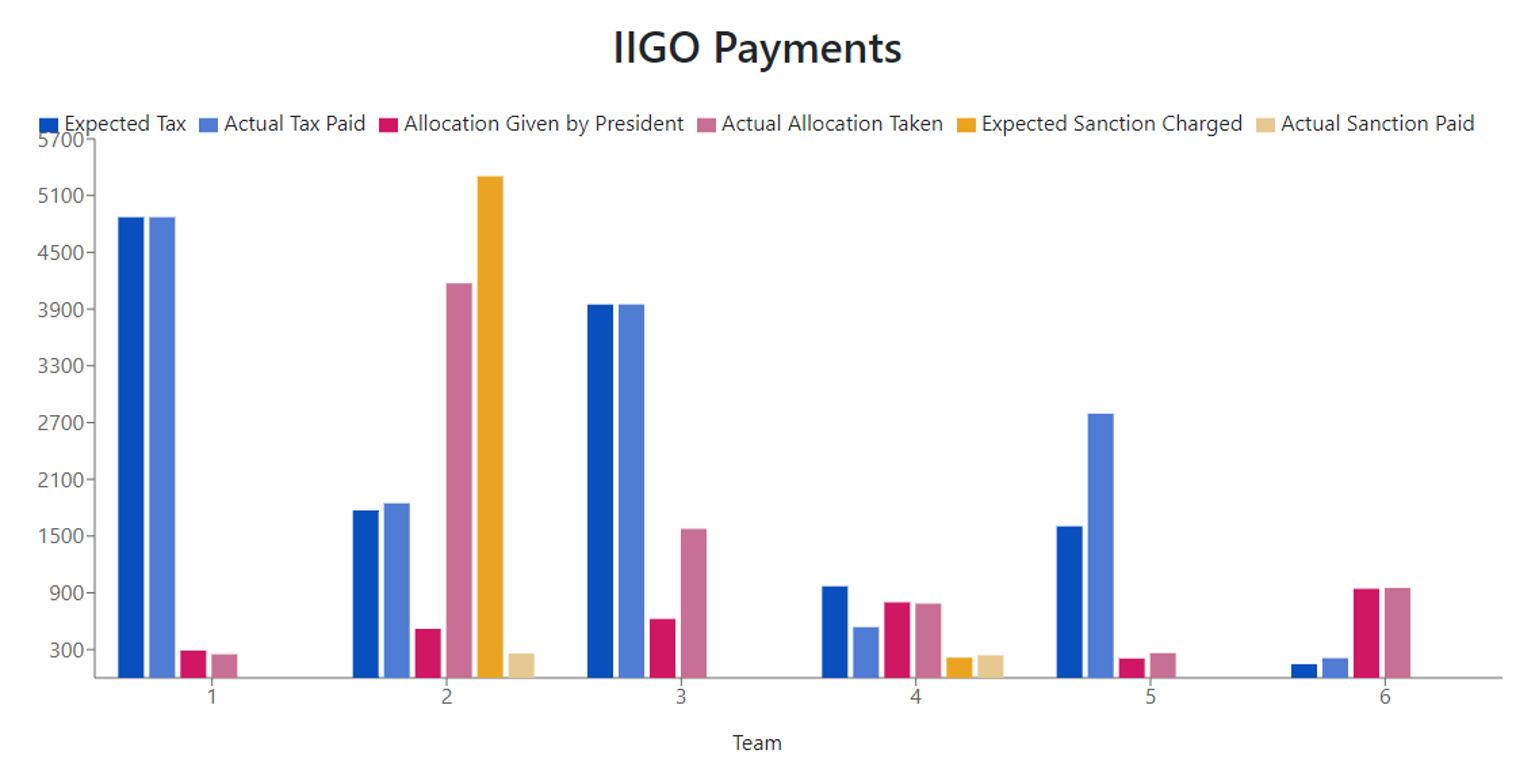
\includegraphics[width=1\textwidth]{15_simulations/images/baseline_iigo_tax_alloc_sanction.png}
    \caption{The tax, allocation and sanction metrics for each Island}
    \label{fig:Simulations:IIGO_numbers}
\end{figure} 
    

\subsection{Baseline IIGO Roles}
\label{subsec:Simulations:baseline:IIGO_roles}

Figure~\ref{fig:Simulations:iigo_roles} show's two possibilites for the IIGO roles that occur when running with the base config. Both result in similar values for the other metrics.

\begin{figure}
    \centering
    \subfigure[More Tyranical]{
      \centering
      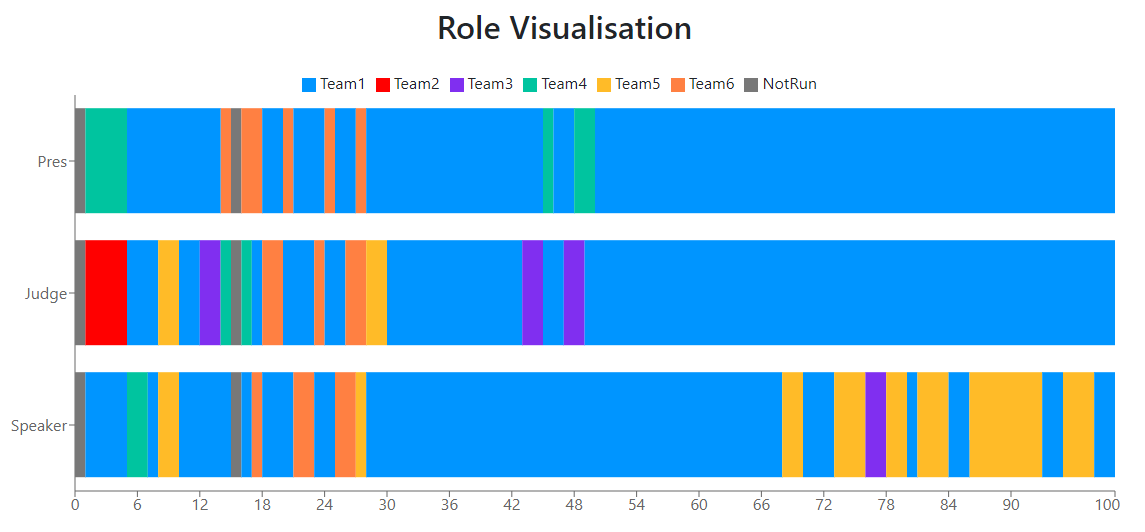
\includegraphics[width=.4\linewidth]{15_simulations/images/baseline_iigo_roles_1.png}
    }
    \subfigure[More Inclusive]{
      \centering
      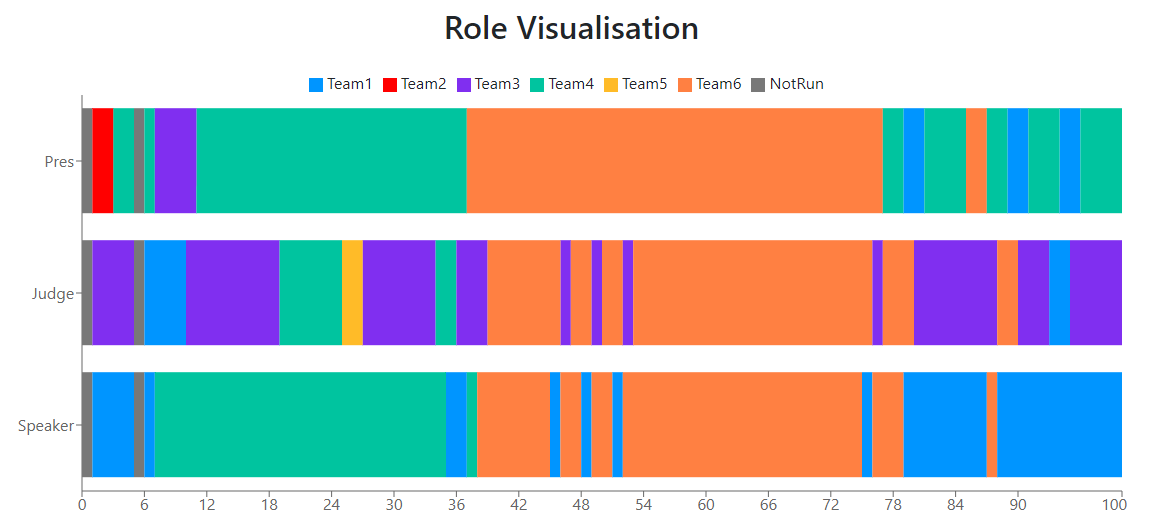
\includegraphics[width=.4\linewidth]{15_simulations/images/baseline_iigo_roles_2.png}
    }
    \caption{Two potential outcomes for role allocations in IIGO}
    \label{fig:Simulations:iigo_roles}
\end{figure}

\subsection{Baseline Gifting}
\label{subsec:Simulations:baseline:trading}

\begin{figure}[H] 
    \centering
    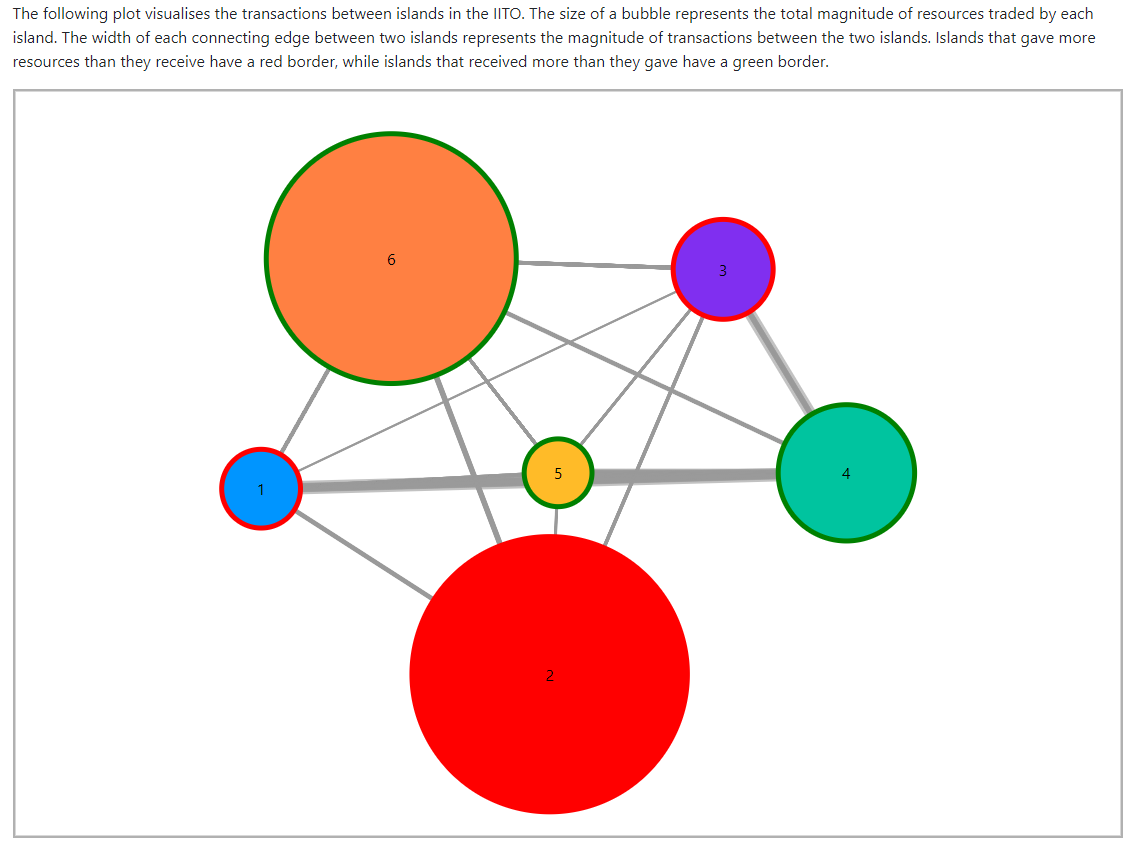
\includegraphics[width=1\textwidth]{15_simulations/images/baseline_gifts.png}
    \caption{A diagram representing the gifts between all islands}
    \label{fig:Simulations:IITO_gifts}
\end{figure} 

Note: If a metric is not of interest to a certain area of exploration it will not be shown.